\chapter{LocText Corpus}\label{chapter:corpus}

\section{Need for a separate corpus}

As mentioned in the previous chapter, the GENIA event corpus or its subset, the BioNLP shared task corpus is not the best corpus to be used for the task of protein-location relation extraction. As pointed out previously, following are some of the issues related to the GENIA event corpus:

\begin{enumerate}

\item Not all the locations mentioned in the GENIA event corpus are subcellular locations. Some of the locations are names of cells or tissues in the body.

\item In some mentions of locations, there are extraneous words in addition to the actual  mention of a subcellular location. These extraneous words takes away the preciseness of the mention of location.

\item Some \textit{Localization} events does not contain an actual mention of subcellular location, i.e., neither the event trigger nor its arguments refers to any subcellular location. The event is annotated only due to the reason that the context gives a clue about the \textit{Localization} event.

\end{enumerate}

To summarize, the GENIA event corpus have some issues and cannot be directly used for the task of protein-location relation extraction. Therefore, there was a need to create a separate corpus dedicated for this task.

\section{LocText}\label{sec:LocTextCorpus}

I, along with my team, annotated a corpus consisting of 100 MEDLINE \cite{medline} abstracts. We called the corpus "LocText". To select the abstracts that contain evidence of subcellular localization of protein, a list of PubMed \cite{pubmed} identifiers, cited by UniprotKB \cite{magrane2011uniprot} protein subcellular localization annotations, was made. From this list, 100 abstracts were chosen randomly. In order to have sufficient taxonomic variation, it was made sure that 50 abstracts belonged to human and 25 abstracts belonged each to budding yeast (\textit{Saccharomyces cerevisiae}) and Arabidopsis (\textit{Arabidopsis thaliana}).

\section{Corpus annotation process and guidelines}

The process of corpus annotation started with random selection of 100 abstracts. The annotation of the corpus was done with the help of \textit{tagtog} \cite{cejuela2014tagtog}. The corpus was annotated for:

\begin{enumerate}
\item Entities
\begin{enumerate}
\item Proteins (including gene and mRNA mentions)
\item Subcellular locations
\item Organisms
\end{enumerate}
\item Relations
\begin{enumerate}
\item Protein - Organism
\item Protein - Subcellular location
\end{enumerate}
\end{enumerate}

\subsection*{Normalization of entities}

Every entity was normalized to a unique identifier in order to have a uniform representation of entities and the relations involving those entities. Protein annotations were normalized to UniprotKB \cite{magrane2011uniprot} identifiers, subcellular localization annotations were normalized to Gene Ontology (GO) \cite{ashburner2000gene} terms and organism annotations were normalized to NCBI Taxonomic \cite{ncbiTaxonomy} identifiers.

\subsection*{Annotation guidelines}
Out of 100 abstracts, 46 abstracts were used to develop the annotation guidelines. The guidelines, along with the full corpus, is available at \url{https://www.tagtog.net/-corpora/loctext}. Some of the important guidelines used during the annotation process are listed as follows:

\begin{itemize}

\item Protein names should be annotated only if the names are found in UniprotKB \cite{magrane2011uniprot} for particular organism.

\item Subcellular locations should be annotated only if these location names are found in GO ontology \cite{ashburner2000gene}.

\item Organism names should be annotated only if the organism name corresponds to rank species, genus or subfamily in NCBI Taxonomy \cite{ncbiTaxonomy}.

\item For all the relations (protein-organism \& protein-location), the context is  important and the relation should not be made without sufficient evidence.

\end{itemize}


\begin{figure}
\centering
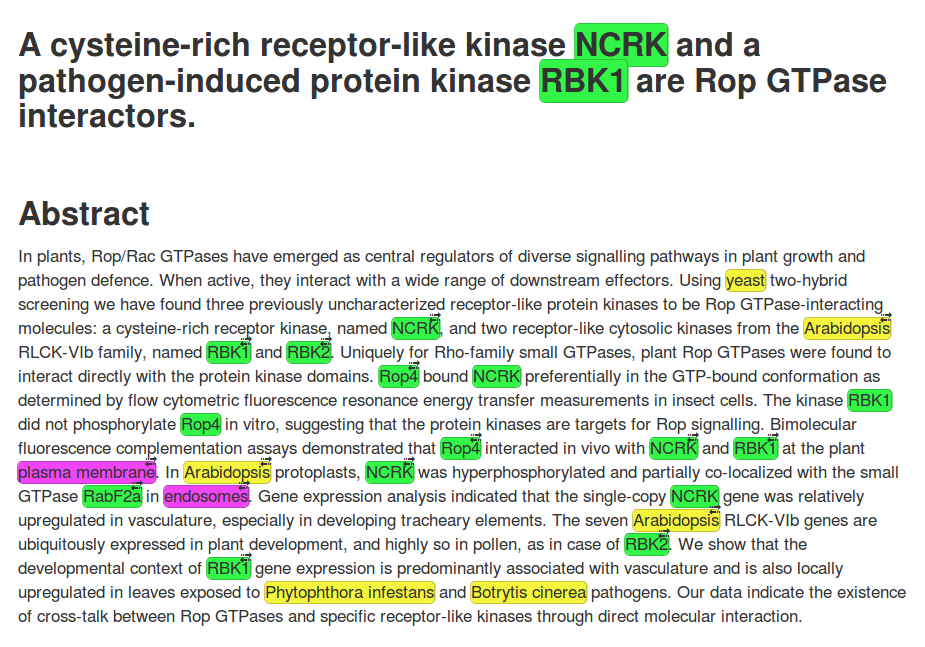
\includegraphics[scale=0.4]{figures/tagtog_screenshot.png}
\caption{Screenshot of an abstract from tagtog annotation tool}\label{fig:tagtogScreenshot}
\end{figure}

Figure \ref{fig:tagtogScreenshot} shows an example abstract annotated in the tagtog annotation tool. Proteins, locations and organisms are highlighted in yellow, green and magenta respectively. The entities, which participates in either protein-organism or protein-location relation, have a double arrow as an additional marking.

\section{Inter-annotator agreement (IAA)}

Inter-annotator agreement is a term quite often used in linguistics. It determines the agreement between different annotators on predefined set of annotated documents. High inter-annotator agreement implies that the annotation guidelines are very clear and different annotators agreed on most of the annotations.

As mentioned earlier, 46 out of 100 abstracts were used for developing annotation guidelines. Remaining 54 abstracts were independently annotated by me and my teammate Tatyana Goldberg using annotation guidelines. The inter-annotator agreement was calculated using annotations from these 54 abstracts. The inter-annotator agreement was denoted by F1 score and it was calculated separately for entity and relation annotations. The F1 score was calculated using following formula:

$$
F1 = \frac{2*X_{AB}*X_{BA}}{X_{AB}+X_{BA}}
$$

where $X_{ij}$ is the fraction of annotations by annotator i matching those of annotator j.

Since the focus of corpus annotation was protein-location relation extraction, the IAA was calculated for annotations of entities, viz. proteins and subcellular locations, and annotations of protein-location relations.

\subsection*{IAA for entities}

Two annotations of the same entity were considered to match if they have the exact same start offsets and end offsets. The IAA between two annotators was F1 score of  96\% and 88\% for protein and location annotations respectively. The combined F1 score for entity types was 94\%.

\subsection*{IAA for relations}

A protein-location relation annotation was defined to match between two annotators if annotations of both the protein and location entity match between the annotators, according to the definition above.

The IAA between two annotators was F1 score of 80\% for protein-location relations.

\section{Important insights from the corpus and publication of results}

% Explain about the results that you published at the BLAH conference
Some important insights were derived from LocText annotation. The annotation of the corpus was done from scratch without actually referring to the annotations present in the knowledge bases like UniProtKB. When the protein-location relations present in the corpus were compared with the information already present in the knowledge bases, it was found out that the corpus has more annotations for same set of documents compared with UniProtKB.

The annotations in LocText were, thus, divided in three categories, viz. \textit{existing}, \textit{more detailed} and \textit{novel}. \textit{Existing} annotations are the ones that are present in knowledge bases already. An annotation was defined as \textit{more detailed} annotation if it provides more information than what is present in the knowledge bases. In the same way, an annotation was defined as \textit{novel} annotation if it is not present in the knowledge bases. The annotations were further subdivided based on whether or not the relationships involve UniprotKB proteins that cite the abstract.

\begin{table}
\centering
\begin{tabular}{|c|c|c|c|c|c|c|}
\hline
\textbf{Category} & \multicolumn{2}{c|}{\textbf{Existing}} & \multicolumn{2}{c|}{\textbf{More detailed}} & \multicolumn{2}{c|}{\textbf{Novel}} \\ 
\hline
\textbf{Citing Protein} & \textbf{Yes} & \textbf{No} & \textbf{Yes} & \textbf{No} & \textbf{Yes} & \textbf{No} \\
\hline
Human & 29 & 15 & 1 & 1 & 14 & 3 \\
Budding Yeast & 22 & 14 & 5 & 3 & 6 & 5 \\
Arabidopsis & 19 & 7 & 5 & 2 & 6 & 7 \\
Other & 2 & 9 & 0 & 0 & 0 & 6 \\
\hline
Subtotal & 72 & 45 & 11 & 6 & 26 & 41 \\
\hline
\textbf{Total} & \multicolumn{2}{c|}{\textbf{117}} & \multicolumn{2}{c|}{\textbf{17}} & \multicolumn{2}{c|}{\textbf{67}} \\ 
 \hline
\end{tabular}
\caption{Comparison of protein-location annotations in LocText with information available in UniProtKB}\label{tab:novelAnnotation}
\end{table}

% Write about observations from table here
As shown in the Fig. \ref{tab:novelAnnotation}, novel or more detailed annotations could be found out for 84 out of 201 (42\%) proteins in 34 abstracts. For example, as seen in Fig. \ref{fig:tagtogScreenshot}, the Arabidopsis protein RabF2a is localized to the endosomes, which at the time of publication of results was not recorded in UniProtKB entry RAF2A\_ARATH.

Therefore, these findings show that the annotations in databases such as UniprotKB aren't complete and there is a considerable room for improvement. The results \cite{goldberg2015linked} were published in the symposium at Biomedical Linked Annotation Hackathon (BLAH) 2015 \cite{blah}. From these results, it can be concluded that manually annotated corpora can contribute novel information about proteins in addition to what is present in the knowledge bases. A case study was presented which proves that the creation of linked annotation resource would contain more annotations. Since the biomedical research community and the natural language processing (NLP) community both undertake the annotations of text with different objectives in mind, linked annotations comprising contributions from both communities could be immensely helpful. In addition, such a linked annotation resource would also create a synergy between the biomedical research community and the natural language processing community.


\section{Corpus statistics}\label{sec:corpusStats}

% Put all the numbers with respect to number of entities, relations and their distribution here. Also, put all the nice graphs that you made here

As stated earlier, the LocText corpus is made by annotating 100 MEDLINE abstracts. Although collectively called as abstracts, the corpus is made by annotating 100 documents and every document has a title part and an abstract part. This section presents an analysis of the annotations from various perspectives, viz. whether the annotation is present in the title or the abstract, the type (protein-location/protein-organism) in case of relation annotations, etc.

\subsection*{Count of entities and relations}

\begin{figure}
\centering
\begin{minipage}{.5\textwidth}
  \centering
  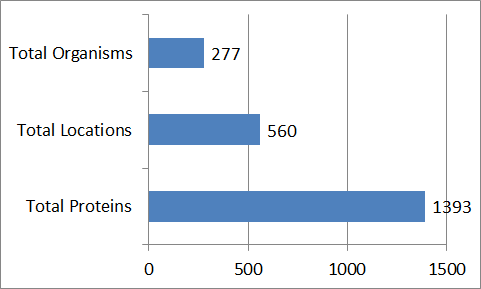
\includegraphics[width=.95\textwidth]{figures/ProtLocOrg_Distribution.png}
  \caption{Entities in LocText corpus}
  \label{fig:LocText_Entities}
\end{minipage}%
\begin{minipage}{.5\textwidth}
  \centering
  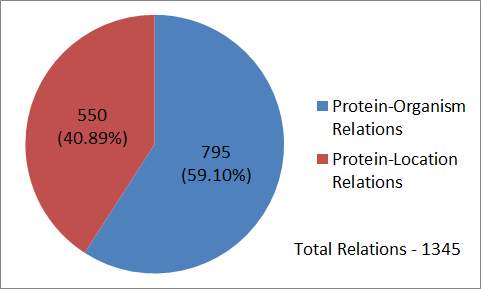
\includegraphics[width=.95\textwidth]{figures/AllRelationsPie.png}
  \caption{Relations in LocText Corpus}
  \label{fig:LocText_Relations}
\end{minipage}
\end{figure}

Fig. \ref{fig:LocText_Entities} and \ref{fig:LocText_Relations} shows the count of entities and relations present in 100 documents of the LocText corpus. As shown in  Fig. \ref{fig:LocText_Entities}, there are 1393 protein, 560 location and 277 organism annotations in the corpus. Similarly, Fig. \ref{fig:LocText_Relations} shows that there are a total of 1395 relations in the corpus, 550 of which are protein-location relations and 795 are protein-organism relations. Protein-organism relations contribute nearly 60\% of the total relations whereas protein-location relations make up remaining 40\%.

\subsection*{Analysis of relations}

\begin{figure}
\centering
\begin{minipage}{.5\textwidth}
  \centering
  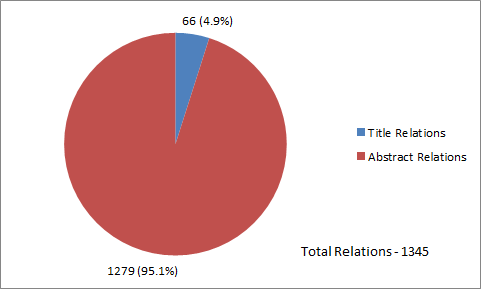
\includegraphics[width=.95\textwidth]{figures/Rel_Title_Abs_Distribution.png}
  \caption{Distribution in corpus}
  \label{fig:Rel_Title_Abs}
\end{minipage}%
\begin{minipage}{.5\textwidth}
  \centering
  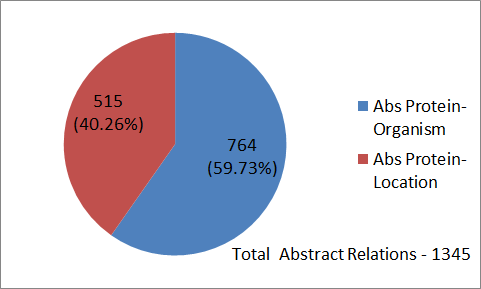
\includegraphics[width=.95\textwidth]{figures/AbsRel_PO_PL_Distribution.png}
  \caption{Distribution in abstract}
  \label{fig:Rel_Abs_PO_PL}
\end{minipage}
\end{figure}

The relations are categorized in two key categories, viz. same-sentence relations and  different-sentence relations. Same-sentence relations are those relations in which both the participating entities lie in the same sentence and different-sentence relations are those relations in which either of the participating entities is in a different sentence. Same-sentence relations can also be defined as intra sentence relations and different-sentence relations can be defined as inter sentence relations.

As seen in the Fig. \ref{fig:Rel_Title_Abs}, only a minor fraction (5\%) of the relations are present in the title while remaining 95\% relations are present in the abstract. The relations that are present in the title are all same-sentence relations since there isn't a single document in the corpus where the title spans more than one sentence. Therefore, the 5\% relations that are present in the title are all same-sentence relations.

Fig. \ref{fig:Rel_Abs_PO_PL} shows the distribution of relations in the abstract according to its type. Of the total relations present in the abstracts, about 40\% are protein-location relations and about 60\% are protein-organism relations. Note that this distribution of protein-location and protein-organism relations is consistent with the distribution in the corpus as a whole (illustrated in Fig. \ref{fig:LocText_Relations}).

\begin{figure}
\centering
\begin{minipage}{.5\textwidth}
  \centering
  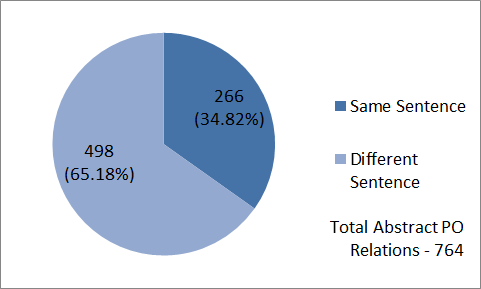
\includegraphics[width=.95\textwidth]{figures/AbsPORels_sent_Distribution.png}
  \caption{Abstract PO Relations}
  \label{fig:Abs_PO_Rel}
\end{minipage}%
\begin{minipage}{.5\textwidth}
  \centering
  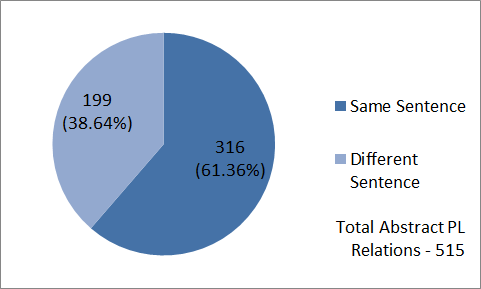
\includegraphics[width=.95\textwidth]{figures/AbsPLRels_sent_Distribution.png}
  \caption{Abstract PL Relations}
  \label{fig:Abs_PL_Rel}
\end{minipage}
\end{figure}


Fig. \ref{fig:Abs_PO_Rel} and \ref{fig:Abs_PL_Rel} shows the distribution of protein-organism (PO) and protein-location(PL) relations into same-sentence relations and different-sentence relations. As shown in Fig. \ref{fig:Abs_PO_Rel}, about 35\% of the PO relations are same-sentence relations and 65\% are different-sentence relations. While in terms of PL relations, \ref{fig:Abs_PL_Rel} shows that about 61.4\% of the PL relations are same-sentence relations and 38.6\% are different-sentence relations.

\begin{figure}
\centering
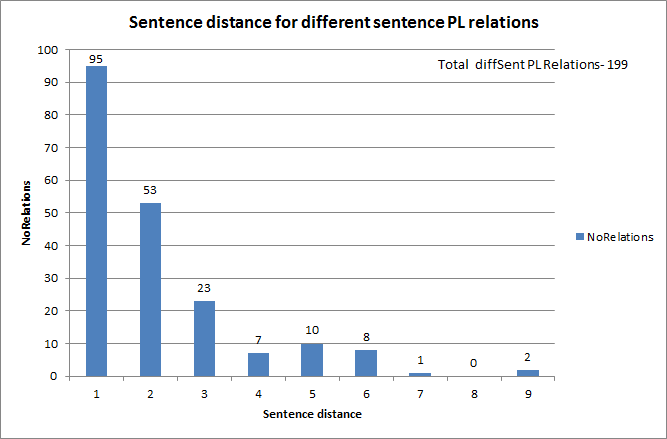
\includegraphics[scale=0.9]{figures/SentenceDistance_PLRel.png}
\caption{Sentence distance for PL Relations}\label{fig:SentDistancePL}
\end{figure}

The relations that are of prime interest are protein-location relations. From previous figures, it is already known that around 60\% of the PL relations in the abstract can be found in the same sentence. Fig. \ref{fig:SentDistancePL} shows how different-sentence PL relations are distributed according to the sentence distance. The different-sentence relations in which the participating entities are in neighboring sentences is said to have a sentence distance of 1. In other words, the sentence distance of 1 indicates that the entities participating in the relation are 1 sentences apart. 

As seen in the Fig. \ref{fig:SentDistancePL}, it is also possible to find the relations with sentence distance 9 which means that the participating entities are 9 sentences apart. However, most of the different sentence relations have lower sentence distance. For example, about 95 out of 199 (47.74\%) different sentence relations are 1 sentences apart.

%TODO need a figure for distribution of PO PL in title as well.

Therefore to summarize the discussion, it can be concluded that 316/515 abstract PL relations (Fig. \ref{fig:Abs_PL_Rel}) and 35 title PL relations are same-sentence relations, which mean that about 351/550 (63.81\%) of total PL relations are same-sentence relations. As seen from  Fig. \ref{fig:SentDistancePL}, 95/199 (47.74\%) different-sentence relations are at the distance of 1. Therefore, a total of 446/550 (81.09\%) PL relations are either same-sentence relations or have a sentence distance of 1. In other words, for about 81\% PL relations, the participating entities are either in the same sentence or in the neighboring sentences. Hence, even if these 81\% relations could be extracted with high accuracy, it would be possible to extract a significant amount of information from the text.

\section{Annotation of full-text articles} \label{sec:full-text}

We decided to annotate some full-text articles in order to compare and contrast the statistics of entities and relations with the abstracts-only corpus. The annotation guidelines developed for annotating abstracts in LocText was used for annotating full-text articles. To add full-text articles, PubMed identifiers for 100 selected abstracts were converted to PMC identifiers \cite{pubmedtopmc}. From this list of PMC identifiers, 4 full-text articles were added to "LocText". These 4 full-text articles would be collectively called as full-text subcorpus in this section.

\begin{figure}
\centering
\begin{minipage}{.5\textwidth}
  \centering
  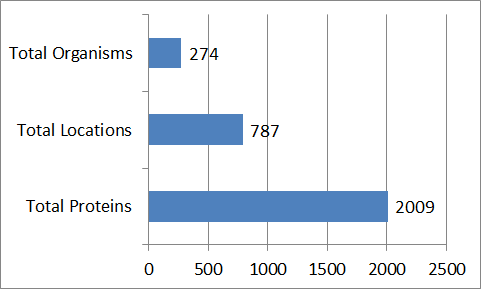
\includegraphics[width=.95\textwidth]{figures/1_FullTextEntities.png}
  \caption{Entities in full-text articles}
  \label{fig:FT_entities}
\end{minipage}%
\begin{minipage}{.5\textwidth}
  \centering
  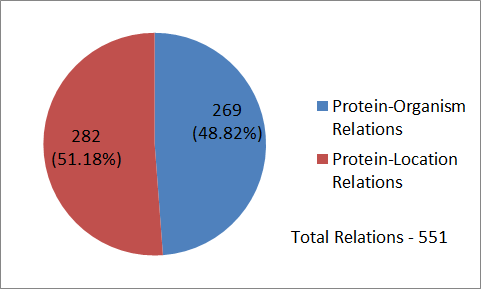
\includegraphics[width=.95\textwidth]{figures/1_FullTextRelationDistribution.png}
  \caption{Relations in full-text articles}
  \label{fig:FT_relations}
\end{minipage}
\end{figure}

As shown in Fig. \ref{fig:FT_entities}, there are 2009 protein entities, 787 location entities and 274 organism entities in the full-text subcorpus. There are a total of 551 relations, of which 269 are protein-organism relations and 282 are protein-location relations. Most of the 282 protein-location relations are repetitive. If duplicate protein-location relations are removed, the number of protein-location relations drops to 86.

\begin{figure}
\centering
\begin{minipage}{.5\textwidth}
  \centering
  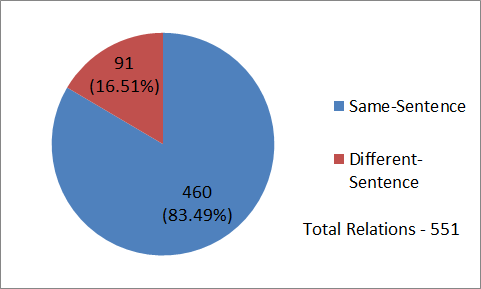
\includegraphics[width=.95\textwidth]{figures/2_FTTotalRelDist.png}
  \caption{Total relations distribution}
  \label{fig:FT_RelDist}
\end{minipage}%
\begin{minipage}{.5\textwidth}
  \centering
  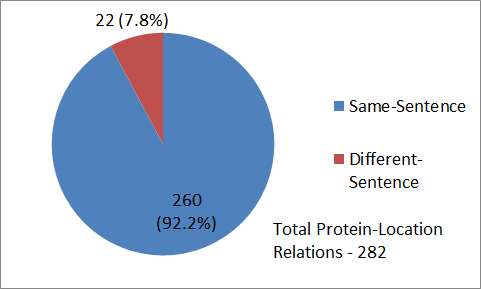
\includegraphics[width=.95\textwidth]{figures/2_FTPLRelDist.png}
  \caption{PL relations distribution}
  \label{fig:FT_PLRelDist}
\end{minipage}
\end{figure}

Fig. \ref{fig:FT_RelDist} and Fig. \ref{fig:FT_PLRelDist} shows the distribution of relations into same-sentence relations and different-sentence relations. As shown in Fig. \ref{fig:FT_RelDist}, around 83.49\% of total relations are same-sentence relations whereas only 16.51\% of total relations are different-sentence relations. The proportion worsens if only protein-location relations are considered. Fig. \ref{fig:FT_PLRelDist} shows that, about 92.2\% of the total protein-location relations are same-sentence relations while remaining 7.8\% are different-sentence relations. This distribution of protein-location relations in the full-text subcorpus is in stark contrast with the abstract subcorpus. While abstract subcorpus had around 40\% different-sentence protein-location relations (see Fig. \ref{fig:Abs_PL_Rel}), the full-text subcorpus has only 7.8\% different-sentence relations.

\section{Linked annotation}

%Write about contribution in BLAH

\begin{figure}
\centering
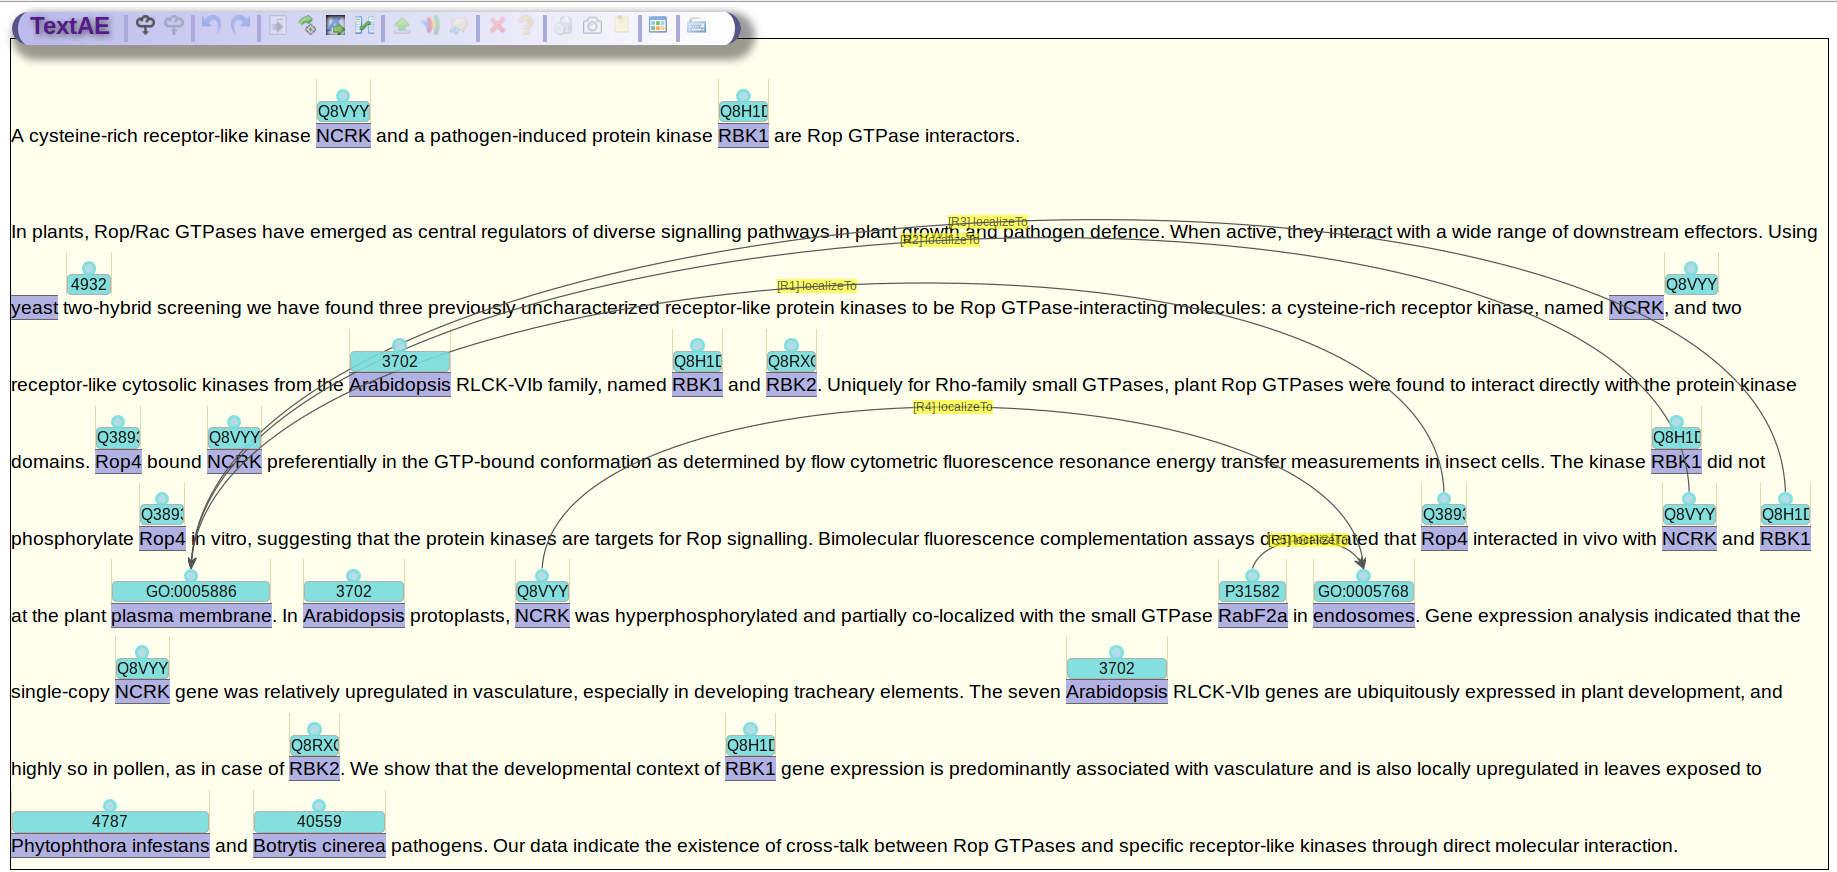
\includegraphics[scale=0.25]{figures/TextAE_Vis.png}
\caption{Visualization of annotations in TextAE}\label{fig:TextAEVis}
\end{figure}

As a part of the efforts to create a \hyperref[http://2015.linkedannotation.org/background]{linked annotation} resource, we also participated in the event BLAH \cite{blah} and the symposium. 

The tagtog annotation web interface stores the annotation in a different format than the format used at the BLAH hackathon. At the hackathon, the data was to be used in PubAnnotation format. PubAnnotation \cite{kim2012pubannotation} is a repository of text annotations and it has its own format to represent the annotation for any article. It also uses a visualization tool TextAE \cite{textae} for visualizing the annotations. Therefore, the data in tagtog JSON format was converted to PubAnnotation JSON format. The code for converting data in tagtog JSON format to PubAnnotation JSON format is available at \url{https://github.com/Aryabhatta/BLAHSubmission} \cite{blahsubmission}. The annotations which are shown in Fig \ref{fig:tagtogScreenshot} are represented as Fig. \ref{fig:TextAEVis} in the TextAE visualization tool. 

The LocText corpus is available for download under \hyperref[https://creativecommons.org/licenses/by/4.0/]{Creative Commons Attribution 4.0} in tagtog format at \url{https://www.tagtog.net/-corpora/loctext}  and in PubAnnotation format at \url{http://pubannotation.org/projects/LocText}.